\documentclass{tufte-handout}
\usepackage{amsmath}
\pagestyle{empty}
\usepackage[utf8]{inputenc}
\usepackage{mathpazo}
\usepackage{booktabs}
\usepackage{microtype}
\usepackage{xcolor}

\usepackage{tikz}
\usetikzlibrary{matrix}
\usetikzlibrary{chains}
\usetikzlibrary{decorations}

\input{vc.tex}

\title{Gorilla--Sea Cucumber Hash}
\author{Thore Husfeldt}
\date{\small Revision \GITAbrHash, \GITAuthorDate}


\begin{document}

\maketitle

\subsection{Description}
This is a simple data mining application that uses hashing to compare protein sequences in order to learn if we are closer (genetically) to a gorilla or a sea cucumber.

\begin{figure}
  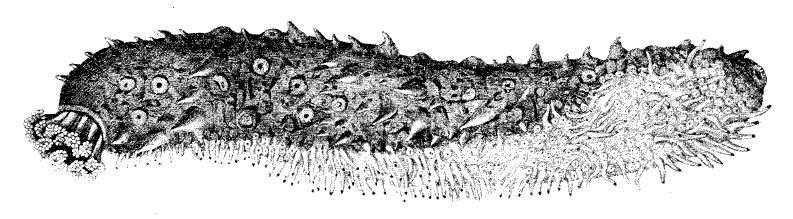
\includegraphics[width=\textwidth]{sea_cucumber.png}
  \caption{A sea cucumber. Ugly bastard.
  Image from \emph{Nordisk familjebok}, 1876.}
\end{figure}

Implement the similarity algorithm described below.
You can use whatever hash function you want, and play around with parameters $k$ and $d$ until you get output that you are biologically comfortable with.
For me, $k=20$ and $d=10000$ works pretty well.
You may need to consult some kind of reference work to remember (or learn) what a dot product is, and how to compute $|p|$, the length of vector $p$.

\subsection{Input}
The input file {\tt HbB\_FASTAs.in} contains proper data from some protein sequence database.
Below are the first few lines of {\tt HbB\_FASTAs.in}.

\begin{fullwidth}
  \begin{quote}
\begin{verbatim}
>Human 2144721 HBHU 4HHB
MVHLTPEEKSAVTALWGKVNVDEVGGEALGRLLVVYPWTQRFFESFGDLSTPDAVMGNPKVKAHGKKVLG
AFSDGLAHLDNLKGTFATLSELHCDKLHVDPENFRLLGNVLVCVLAHHFGKEFTPPVQAAYQKVVAGVAN
ALAHKYH
>Gorilla 232230
MVHLTPEEKSAVTALWGKVNVDEVGGEALGRLLVVYPWTQRFFESFGDLSTPDAVMGNPKVKAHGKKVLG
AFSDGLAHLDNLKGTFATLSELHCDKLHVDPENFKLLGNVLVCVLAHHFGKEFTPPVQAAYQKVVAGVAN
ALAHKYH
...
\end{verbatim}
\end{quote}
\end{fullwidth}

The protein sequence for Human takes up three lines, from {\tt MVHL} to {\tt KYH}.
It contains a list of amino acids, coded as alphabetic letters.
Then, after the next {\tt >} symbol, the file continues with the next species, Gorilla.
Ignore things like {\tt 2144721 HBHU 4HHB} -- I have no idea what that stuff even means!

\subsection{Output}

For each pair of organisms, output a number between $0$ and $1$ that describes their similarity.
If you did everything right, organisms like Human and Gorilla should be judged more similar than Cow and Sea cucumber, which is consistent with our knowledge of evolution.


\subsection{Similarity test based on hashing}

For integer $k$, a \emph{$k$-gram} of a string is a substring of length $k$.
Clearly, every string of length $n$ has at most $n-k$ such $k$-grams, but it may have fewer because of repetitions.
For instance, the $2$-grams of ABABAA are AB, BA, and AA.
Both AB and BA appear twice.

For integer $d$, let $h$ be a hash function that maps the set of $k$-grams to the integers $\{0,\ldots,d-1\}$ .
For example, in Java, you could define $h(S)$ as
{\tt (S.hashcode() \% d) }.
Given a string $S$, define for each $i$ with $0\leq i< d$ the value $p_i$ as the number of $k$-grams $T$ of $S$ for which $h(T) = i$.
The resulting $d$-dimensional vector $p=(p_0,\ldots,p_{d-1})$ is called the \emph{profile} of $S$.
We then define the \emph{similarity} of two strings with profiles $p$ and $q$ as
\[
    \frac{p\cdot q}{\left|p\right| \left|q\right|}\,,
\]
where $p\cdot q$ is the dot product\sidenote{The dot product is sometimes called the scalar product or inner product.}
of $p$ and $q$, and $|p|$ is the (Euclidean) length of $p$.

\medskip
Why is this this a reasonable definition of similarity?
First, two identical strings have the same profile.
More interestingly, two similar strings will have similar profiles: ABACADABRA and BABABLACKSHEEP contain AB the same number of times, both of which contribute to the profile index counting $h(\text{AB})$.
Assuming uniform hashing, no other $2$-grams are likely to get the same hash value, so the profile index is roughly the same.
We can then define two profile vectors as similar if they ``point in the same direction,''
which means that the angle between them is small.
Recall that the angle $\alpha$ between two vectors $p$ and $q$ is defined as \(
  \cos \alpha =
    (p\cdot q)/(\left|p\right| \left|q\right|).
    \)
Further recall that the trigonometric function cosine transforms an angle into a number between $-1$ and $+1$, with $\cos\alpha$ being close to $1$ when the angle between $p$ and $q$ is very small.

\subsection{Requirements}

Your output will depend on your choice of hash function and several parameters, so I cannot provide sample output to help you evaluate the correctness of your code.
You probably need a few lines of code for basic operations on Euclidean vectors (length, angle).
That part you should test, even if you didn't write it yourself.\sidenote{Actually, \emph{in particular} if you didn't write it yourself.}

\subsection{Deliverables}

\begin{enumerate}
  \item The java source code for your implementation
  \item A report in PDF.
  Use the report skeleton on the next page.
  \end{enumerate}

\subsection{Background and further reading}

Is this really how it’s done?
Well, close enough.
In particular, techniques for comparing documents (for
example to detect near-duplicates for web search engine
reporting, data mining, or fraud dectection) are based on
comparing hash values.
The details are slightly different---if you want to read up on this, start with Wikipedia’s article on min-wise independent hashing.

Why don't we just compute the profiles of the $k$-grams themselves, instead of their hash values?
The problem is that the profiles become too large.
Assume for a moment that there are only 24 letters in the alphabet.
Then there are $24^k$ different $k$-grams, and your profile vector $p$ would be $24^k$-dimensional.
Good luck storing that on your machine for $k=20$, say!
Also, most of the entries in $p$ would end up being $0$ anyway.
With hashing, you need only $d$ dimensions.
This is a prototypical hashing application:
Avoid storing a sparse table by hashing it into a much smaller table without losing too much information.

\medskip
For comparing protein sequences, one normally uses a more
precise distance estimate called the \emph{Levenshtein} distance,
sometimes called \emph{edit distance}.
For that particular distance there's actually a better algorithm called \emph{dynamic
programming}, which works fast enough for such small inputs.
The same idea is used by your word processor’s spell
checker.
This is the basis of another programming exercise that you may be exposed to in another course.

\newpage
\section{Gorilla--Sea Cucumber Hash Report}

by Alice Cooper and Bob Marley\sidenote{Complete the report by filling
  in your names, filling in the parts marked $[\ldots]$ and changing other parts wherever necessary.
  (For instance, the numbers is the tables are nonsense right now.)
  Remove the sidenotes in your final hand-in.}

  \subsection{Results}

  The following table gives the similarity between each pair of species as a number between 0 and 1, higher values meaning ``more similar.''
  We have used the hash function $h(S) = [\ldots]$ with  $d=[\ldots]$ and $k$-grams of length $k=[\ldots]$.
  As can be seen, the species closest to us is the $[\ldots]$.

  \bigskip\noindent
  {\small\sf
  \begin{tabular}{rcccccccccccc}
  \toprule
    &Human
    &Gorilla
    &Monkey
    &Horse
    &Deer
    &Pig
    &Cow
    &Gull
    &Trout
    &R. Cod
    &Lamprey
    &Sea Cuc.
    \\\midrule
  Human & 1 & 0.534 & $[\ldots]$ \\
  Gorilla &\\
  $[\ldots]$\\
  \bottomrule
  \end{tabular}
  }


  \subsection{Tests}

  Our static method {\tt double cos\_angle(int[] p, int[] q)} computes the cosine of the angle of two vectors of the same length $d$.
  We have tested it on the following examples:

  \bigskip\noindent
{ \small\sf
  \begin{tabular}{cccc}
  \toprule
  $p$     & $q$     & $d$ & value returned \\\midrule
  $(0,1)$ & $(0,1)$ & $2$ & $\pi$ \\
  $(0,1)$ & $(0,2)$ & $2$ & $4$\\
  $(0,1)$ & $(1,0)$ & $2$ & $[\ldots]$\\
  $(0,1)$ & $(0,-1)$ & $2$ & $[\ldots]$\\
  $(0,\ldots,0,1)$ & $(1,0,\ldots,0)$ & $1000$ & $[\ldots]$\\
  $[\ldots]$ \\
  \bottomrule
  \end{tabular}
}

\bigskip
  Similarly, our static method {\tt length(int[] p)} computes $[\ldots]$.

\end{document}
